%\begin{name}
%	{Biên soạn: Thầy Nguyễn Cường  \& Phản biện: Thầy Dương Xuân Lợi}
%	{Đề chuẩn hóa số 3}
%\end{name}
\caulc
\Opensolutionfile{ans}[ans/ans-cau-TN-chuanhoa-3]
\begin{ex}%[De-chuan-hoa-so-3]%[Nguyễn Cường]%[1D6N3-2]
	Tập xác định của hàm số $y=\log 2024x$ là
	\choice
	{\True $\mathscr{D}=(0;+\infty)$}
	{$\mathscr{D}=[0;+\infty)$}
	{$\mathscr{D}=\mathbb{R}$}
	{$\mathscr{D}=(2024;+\infty)$}
	\loigiai{
		Điều kiện xác định của hàm số là $2024x>0\Leftrightarrow x>0$.\\
		Vậy tập xác định của hàm số là $\mathscr{D}=(0;+\infty)$.
	}
\end{ex}
\begin{ex}%[De-chuan-hoa-so-3]%[Nguyễn Cường]%[1D6N4-2]
	Phương trình $7^x=5$ có nghiệm là 
	\choice
	{$x=\log_57$}
	{\True $x=\log_75$}
	{$x=7^5$}
	{$x=5^7$}
	\loigiai{
		Ta có $7^x=5\Leftrightarrow x=\log_75$.
	}
\end{ex}
\begin{ex}%[De-chuan-hoa-so-3]%[Nguyễn Cường]%[1D6H4-3]
	Tập nghiệm của bất phương trình $\log_{\tfrac{1}{2}}(x-5)\ge -2$ là
	\choice
	{$(5;9)$}
	{$[9;+\infty)$}
	{$(-\infty;9]$}
	{\True $(5;9]$}
	\loigiai{
		Điều kiện $x-5>0\Leftrightarrow x>5$.\\
		Khi đó, $\log_{\tfrac{1}{2}}(x-5)\ge -2\Leftrightarrow x-5\le \left(\dfrac{1}{2}\right)^{-2}\Leftrightarrow x-5\le 4\Leftrightarrow x\le 9$.\\
		Vậy tập nghiệm của bất phương trình là $(5;9]$.
	}
\end{ex}
\begin{ex}%[De-chuan-hoa-so-3]%[Nguyễn Cường]%[1D6N4-4]
	Nếu $\log x=2\log7-\log5$ thì
	\choice
	{$x=\dfrac{14}{5}$}
	{$44$}
	{\True $x=\dfrac{49}{5}$}
	{$2$}
	\loigiai{
		Điều kiện $x>0$.\\
		Ta có $\log x=2\log7-\log5\Leftrightarrow \log x=\log 7^2-\log 5\Leftrightarrow\log x=\log\dfrac{49}{5}$.\\
		Vậy $x=\dfrac{49}{5}$.
	}
\end{ex}

\begin{ex}%[De-chuan-hoa-so-3]%[Nguyễn Cường]%[1D6N3-3]
	\immini 
	{
	Đường cong hình bên là đồ thị của hàm số nào dưới đây?
	\choice
	{$y=2^x$}
	{$y=\log_2x$}
	{\True $y=\log_{\tfrac{1}{2}}x$}
	{$y=\left(\dfrac{1}{2}\right)^x$}
}
{
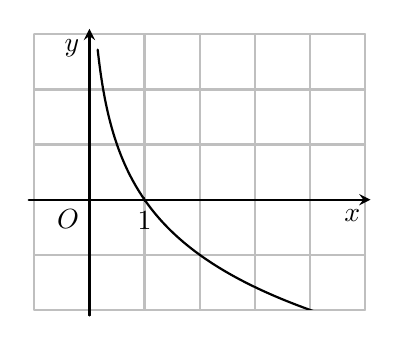
\begin{tikzpicture}[line join=round, line cap=round,>=stealth,thick,scale=0.7]
	\draw[gray!50,xstep = 1, ystep = 1] (-1,-2) grid (5,3);
	\draw[->] (-1.1,0)--(5.1,0) node[below left] {$x$};
	\draw[->] (0,-2.1)--(0,3.1) node[below left] {$y$};
	\draw (0,0) node [below left] {$O$};
	\foreach \x/\nx in {1/1}
	\draw[thin] (\x,1pt)--(\x,-1pt) node [below] {$\nx$};
	\begin{scope}
		\clip (-1,-2) rectangle (5,3);
		\draw[samples=200,domain=0.15:5,smooth,variable=\x] plot (\x,{ln((\x))/ln(0.5)});
	\end{scope}
\end{tikzpicture}
}
	\loigiai{
		Hàm số xác định trên $(0;+\infty)$.\\
		Hàm số nghịch biến trên khoảng $(0;+\infty)$ nên cơ số $a\in (0;1)$.\\
		Vậy hàm số $y=\log_{\tfrac{1}{2}}x$ có đồ thị như hình vẽ.
	}
\end{ex}

\begin{ex}%[De-chuan-hoa-so-3]%[Nguyễn Cường]%[1D9H1-3]
	Hai bệnh nhân M và N bị nhiễm vi rút cúm H5N1. Biết rằng xác suất bị biến chứng nặng của bệnh nhân M là $0{,}05$ và của bệnh nhân N là $0{,}1$. Khả năng bị biến chứng nặng của hai bệnh nhân là độc lập. Tính xác suất của biến cố \lq\lq Bệnh nhân M bị biến chứng nặng, bệnh nhân N không bị biến chứng nặng\rq\rq.
	\choice
	{\True $0{,}045$}
	{$0{,}005$}
	{$0{,}095$}
	{$0{,}855$}
	\loigiai{
	Gọi $A$ là biến cố \lq\lq Bệnh nhân M bị biến chứng nặng\rq\rq. Ta có $\mathrm{P}(A)=0{,}05$ và $P(\overline{A})=0{,}95$.\\
	Gọi $B$ là biến cố \lq\lq Bệnh nhân N bị biến chứng nặng\rq\rq. Ta có $\mathrm{P}(B)=0{,}1$ và $P(\overline{B})=0{,}9$.\\
	Do $A$ và $\overline{B}$ độc lập nên xác suất bệnh nhân M bị biến chứng nặng, bệnh nhân N không bị biến chứng nặng là $$\mathrm{P}(A\overline{B})=\mathrm{P}(A)\cdot\mathrm{P}(\overline{B})=0{,}05\cdot 0{,}9=0{,}045.$$
	}
\end{ex}


\begin{ex}%[De-chuan-hoa-so-3]%[Nguyễn Cường]%[1D7N2-1]
	Đạo hàm của hàm số $y=x^4-3x^2-5x+2017$ là
	\choice
	{$y'=x^3-6x-5$}
	{\True $y'=4x^3-6x-5$}
	{$y'=4x^3-6x+2017$}
	{$y'=4x^3+6x-5$}
	\loigiai{
		Ta có $y'=4x^3-6x-5$.
	}
\end{ex}
\begin{ex}%[De-chuan-hoa-so-3]%[Nguyễn Cường]%[1D7H2-1]
	Đạo hàm của hàm số $y=\dfrac{2x+1}{1-x}$ là	
	\choice
	{$y'=\dfrac{-4x+1}{(1-x)^2}$}
	{$y'=\dfrac{-3}{(1-x)^2}$}
	{\True $y'=\dfrac{3}{(1-x)^2}$}
	{$y'=\dfrac{4x-1}{(1-x)^2}$}
	\loigiai{
		Tập xác định $\mathscr{D}=\mathbb{R}\setminus \{1\}$.\\
		Ta có 
		\allowdisplaybreaks
		\begin{eqnarray*}
			y'&=&\dfrac{(2x+1)'(1-x)-(1-x)'(2x+1)}{(1-x)^2}\\
			&=&\dfrac{2(1-x)-(-1)(2x+1)}{(1-x)^2}\\
			&=&\dfrac{2-2x+2x+1}{(1-x)^2}\\
			&=&\dfrac{3}{(1-x)^2}.
		\end{eqnarray*}
		Vậy $y'=\dfrac{3}{(1-x)^2}$.
	}
\end{ex}

\begin{ex}%[De-chuan-hoa-so-3]%[Nguyễn Cường]%[1D7N2-3]
	Hệ số góc của tiếp tuyến với đồ thị hàm số $y=\sin x+1$ tại điểm có hoành độ $x_0=\dfrac{\pi}{3}$ là
	\choice
	{$k=-\dfrac{\sqrt{3}}{2}$}
	{$k=\dfrac{\sqrt{3}}{2}$}
	{$k=-\dfrac{1}{2}$}
	{\True $k=\dfrac{1}{2}$}
	\loigiai{
		Ta có $y'=\cos x$.\\
		Khi đó hệ số góc của tiếp tuyến với đồ thị hàm số $y=\sin x+1$ tại điểm có hoành độ $x_0=\dfrac{\pi}{3}$ là $$k=y'\left( \dfrac{\pi}{3} \right)=\cos \dfrac{\pi}{3}=\dfrac{1}{2}.$$
		Vậy $k=\dfrac{1}{2}$.
	}
\end{ex}



\begin{ex}%[De-chuan-hoa-so-3]%[Nguyễn Cường]%[1H8H4-3]
	Cho hình chóp $S.ABCD$ có đáy $ABCD$ là hình thoi tâm $I$, cạnh bên $SA$ vuông góc với đáy. Xác định góc giữa hai mặt phẳng $(SBD)$ và $(ABCD)$.
	\choice
	{\True $\widehat{SIA}$}
	{$\widehat{SBA}$}
	{$\widehat{SIC}$}
	{$\widehat{SDA}$}
	\loigiai{
		\immini{
			Do $SA\perp (ABCD)$ nên $SA\perp BD$.\\
			$AI\perp BD$ do $ABCD$ là hình thoi.\\
			Suy ra $BD\perp (SAI)$, mà $SI\subset (SAI)$ nên $BD\perp SI$.\\
			Ta có $\heva{&(SBD)\cap (ABCD)=BD\\& SI\perp BD\\& AI\perp BD} $ \\$\Rightarrow \left((SBD),(ABCD)\right)=(AI,SI)=\widehat{SIA}$.\\
			Vậy số đo góc giữa hai mặt phẳng $(ABCD)$ và $(SBD)$ là $\widehat{SIA}$.
		}
		{
\begin{tikzpicture}[font=\footnotesize,line join=round, line cap=round, >=stealth,scale=0.8]
	\foreach \x/\y/\pos in {0/0/A, -1.5/-1.7/B, 4/0/D} \path ($(\x,\y)$) coordinate (\pos);
	\path ($(B)+(D)$) coordinate (C)
	($(B)!1/2!(D)$) coordinate (I)
	($(A)+(0,3)$) coordinate (S);
	\draw[dashed] (D)--(B)--(A)--(D) (I)--(S)--(A)--(C);
	\draw (C)--(S)--(B)--(C)--(D)--(S);
	\foreach \x/\pos in {S/90, A/180, B/-150, C/-30, D/-30,I/-90} \fill (\x) circle(1pt) node[{shift=(\pos:0.25)}]{$\x$};
	\draw pic[draw,angle radius=2mm] {right angle = S--A--C};
\end{tikzpicture}
		}
	}
\end{ex}



\begin{ex}%[De-chuan-hoa-so-3]%[Nguyễn Cường]%[1H8H5-4]
	Cho hình chóp $ S.ABC $ có đáy $ ABC $ là tam giác cân tại $ A $, cạnh bên $ SA $ vuông góc với đáy. Gọi $ M $ là trung điểm của cạnh $ BC $. Khoảng cách giữa hai đường thẳng $ SA $ và $ BC $ là độ dài đoạn thẳng nào sau đây?
	\choice
	{$AC$}
	{$AB$}
	{\True $AM$}
	{$SM$}
	\loigiai{
		\immini{
			Ta có $ SA\perp (ABC) $ suy ra $ SA \perp AM $.\\
			Hơn nữa tam giác $ ABC $ cân tại $ A $ suy ra $ AM \perp BC $.\\
			Vậy đoạn vuông góc chung giữa $ SA $ và $ BC $ là $ AM $.
		}{
\begin{tikzpicture}[scale=0.7,>=stealth, font=\footnotesize, line join=round, line cap=round]
\coordinate (A) at (-2,0);
\coordinate (B) at (0,-2);
\coordinate (C) at (3,0);
\coordinate (S) at ($(A)+(0,4)$);
\path 
($(B)!.5!(C)$)coordinate(M)
;
\draw(S)--(A) (S)--(B) (S)--(C) (B)--(C) (A)--(B);
\draw[dashed,thin](M)--(A)--(C);
\pic[draw,thin,angle radius=2mm] {right angle = S--A--B} pic[draw,thin,angle radius=2mm] {right angle = S--A--C};
\foreach \i/\g in {S/90,A/180,B/-90,C/0,M/-30}{\draw[fill=black](\i) circle (1.5pt) ($(\i)+(\g:3mm)$) node[scale=1]{$\i$};}
\end{tikzpicture}
	}	
	}
\end{ex}

\begin{ex}%[De-chuan-hoa-so-3]%[Nguyễn Cường]%[1H8H5-2]
	Cho tứ diện $ABCD$ có $AC=a$, $BD=3a$ và $AC$ vuông góc với $BD$. Gọi $M$, $N$ lần lượt là trung điểm của các cạnh $AD$ và $BC$. Khi đó, độ dài đoạn thẳng $MN$ là
	\choice
	{\True $ \dfrac{a\sqrt{10}}{2}$}
	{$ \dfrac{3a\sqrt{2}}{2}$}
	{$ \dfrac{a\sqrt{6}}{2}$}
	{$ \dfrac{2a\sqrt{3}}{3}$}
	\loigiai{
		\immini{
			Gọi $P$ là trung điểm của $CD$.\\
			Khi đó $ PN $ là đường trung bình của $ \triangle BCD$, suy ra $PN \parallel BD$, $NP=\dfrac{1}{2}BD=\dfrac{3a}{2}$.\\
			Tương tự $MP\parallel AC$ và $MP=\dfrac{1}{2}AC=\dfrac{a}{2}$.\\
			Suy ra tam giác $MNP$ vuông tại $P$.\\
			Theo định lý Pythagore ta có
			$$MN=\sqrt{MP^2+NP^2}=\dfrac{a\sqrt{10}}{2}.$$	
		}{
\begin{tikzpicture}[font=\footnotesize,line join=round, line cap=round, >=stealth,scale=0.8]
	\foreach \x/\y/\pos in {0/0/B, 1/-2/C, 5/0/D} \path ($(\x,\y)$) coordinate (\pos);
	\path 
	($(B)+(2,3)$) coordinate (A)
	($(A)!.5!(D)$)coordinate(M)
	($(C)!.5!(B)$)coordinate(N)
	($(D)!.5!(C)$)coordinate(P)
	;
	\draw[dashed] (B)--(D) (M)--(N)--(P)
	;
	\draw 
	(A)--(B)--(C)--(D)--cycle
	(A)--(C) (M)--(P)
	;
	\foreach \x/\pos in {A/90, B/-150, C/-90,D/30,M/30,N/180,P/-30} \fill (\x) circle(1pt) node[{shift=(\pos:0.25)}]{$\x$};
\end{tikzpicture}
	}	
	}
\end{ex}
\Closesolutionfile{ans}
\indapan{7}{ans/ans-cau-TN-chuanhoa-3}

\cauds
\Opensolutionfile{ans}[ans/ans-cau-DS-chuanhoa-3]

\begin{ex}%[De-chuan-hoa-so-3]%[Nguyễn Cường]%[1D7H3-2]
	Cho hàm số $y=16 \cos x +17 \sin x$. Xét tính đúng sai của các mệnh đề sau 
	\choiceTF 
	{\True $y\left(\dfrac{\pi}{4}\right)=\dfrac{33\sqrt{2}}{2}$}
	{$y'=16\sin x+17\cos x$}
	{\True $y''=-16\cos x-17\sin x$}
	{$y''+y=1$}
	\loigiai{
		\begin{itemchoice}
			\itemch Ta có $y\left(\dfrac{\pi}{4}\right)=17\cos\dfrac{\pi}{4}+16\sin\dfrac{\pi}{4}=\dfrac{33\sqrt{2}}{2}$.
			\itemch $y'=-16 \sin x +17 \cos x$.
			\itemch $y''=-16 \cos x -17 \sin x$.
			\itemch $y''+y=16 \cos x +17 \sin x -16 \cos x -17 \sin x =0$.
		\end{itemchoice}
	}
\end{ex}
\begin{ex}%[De-chuan-hoa-so-3]%[Nguyễn Cường]%[1D7V2-5]
	Cho hàm số $y=f(x)=x^3-3x^2+1$ có đồ thị $(C)$ và đường thẳng $d\colon =-\dfrac{1}{9}x+5$. Xét tính đúng sai của các mệnh đề sau
	\choiceTF
	{\True Điểm $M(3;1)$ thuộc đồ thị $(C)$}
	{\True $y'=3x^2-6x$}
	{Tiếp tuyến của đồ thị $(C)$ vuông góc với đường thẳng $d$ có hệ số góc là $k=-\dfrac{1}{9}$}
	{Có một đường tiếp tuyến với đồ thị $(C)$ mà tiếp tuyến vuông góc với đường thẳng $d$}
	\loigiai{ 

		\begin{itemchoice}
	\itemch Với $x=3$, ta có $y=1$. Do đó điểm $M(3;1)$ thuộc đồ thị $(C)$.
	\itemch Đạo hàm $y'=3x^2-6x$.
	\itemch Do tiếp tuyến vuông góc với đường thẳng $d\colon y=-\dfrac{1}{9}x+5$ nên hệ số góc của tiếp tuyến $k=9$.
	\itemch 		
	\begin{itemize}
		\item Đạo hàm $y'=3x^2-6x$.
		\item Do tiếp tuyến vuông góc với đường thẳng $d\colon y=-\dfrac{1}{9}x+5$ nên hệ số góc của tiếp tuyến $k=9$.
		\item Ta có  $y'=k \Leftrightarrow 3x^2-6x=9 \Leftrightarrow \hoac{&x= -1\\&x=3.}$
		\item Với $x=-1 \Rightarrow y= -3 \Rightarrow M(-1;-3)$.\\
		Với $x=3 \Rightarrow y= 1 \Rightarrow M(3;1)$.
		\item Vậy có $2$ phương trình tuyến tuyến: $y=9x+6$; $y=9x-26$.
	\end{itemize}
\end{itemchoice}
}
\end{ex}
\begin{ex}%[De-chuan-hoa-so-3]%[Nguyễn Cường]%[1H8H2-2]%[1H8H2-3]%[1H8H6-1]
	Cho tứ diện $S.ABC$ có $ABC$ là tam giác vuông tại $B$ và $SA\perp (ABC)$. Gọi $AH$ là đường cao của tam giác $SAB$. Xét tính đúng sai của các mệnh đề sau
	\choiceTF
	{\True $SA\perp BC$}
	{\True $AH\perp BC$}
	{\True $AH\perp SC$}
	{Góc giữa đường thẳng $SC$ và mặt phẳng $(SAB)$ là $\widehat{CSA}$}
	\loigiai{
		\immini{\begin{itemize}
				\item $BC\perp SA$ do $SA\perp (ABC)$. 
				\item $\triangle ABC$ vuông tại $B$ $\Rightarrow BC\perp AB$\\
				$\heva{&BC\perp AB\\& BC\perp SA}\Rightarrow BC\perp (SAB) \Rightarrow BC\perp AH$.
				\item $\heva{&AH\perp SB\\& AH\perp BC}\Rightarrow AH\perp (SBC)\Rightarrow AH \perp SC$.
			\end{itemize}
		}
		{
			\begin{tikzpicture}[scale=0.7,>=stealth, font=\footnotesize, line join=round, line cap=round]
				\coordinate (A) at (-2,0);
				\coordinate (B) at (0,-2);
				\coordinate (C) at (3,0);
				\coordinate (S) at ($(A)+(0,4)$);
				\path 
				($(S)!.4!(B)$)coordinate(H)
				;
				\draw(S)--(A) (S)--(B) (S)--(C) (B)--(C) (H)--(A)--(B);
				\draw[dashed,thin](A)--(C);
				\pic[draw,thin,angle radius=2mm] {right angle=S--A--B} pic[draw,thin,angle radius=2mm] {right angle=S--A--C};
				\foreach \i/\g in {S/90,A/180,B/-90,C/0,H/30}{\draw[fill=black](\i) circle (1.5pt) ($(\i)+(\g:3mm)$) node[scale=1]{$\i$};}
			\end{tikzpicture}
		}
	\noindent
		\begin{itemchoice}
		\itemch $BC\perp SA$ do $SA\perp (ABC)$.
		\itemch Ta có $BC\perp (SAB) \Rightarrow BC\perp AH$.
		\itemch $AH\perp (SBC)\Rightarrow AH \perp SC$.
		\itemch Ta có $SB$ là hình chiếu vuông góc của $SC$ trên mặt phẳng $(SAB)$.\\
		Do đó, góc giữa đường $SC$ và mặt phẳng $(SAB)$ là $\widehat{CSB}$.
	\end{itemchoice}
	}
\end{ex}
\begin{ex}%[De-chuan-hoa-so-3]%[Nguyễn Cường]%[1H8H7-2]%[1H8V2-2]
	Cho tứ diện $OABC$ có các cạnh $OA$, $OB$, $OC$ đôi một vuông góc với nhau. Gọi $H$ là trực tâm của tam giác $ABC$. Xét tính đúng sai của các mệnh đề sau
	\choiceTF
	{\True $OA\perp (OBC)$}
	{$V_{OABC}=\dfrac{1}{3}\cdot OA\cdot OB\cdot OC$}
	{\True $OH\perp (ABC)$}
	{\True $\dfrac{1}{OH^2}=\dfrac{1}{OA^2}+\dfrac{1}{OB^2}+\dfrac{1}{OC^2}$}
	\loigiai{
		\immini{
			Gọi $K$ và $L$ lần lượt là chân đường cao kẻ từ $C$ và $B$ của tam giác $ABC$.
			\begin{itemize}
				\item $\heva{&OA\perp OB\\&OA\perp OC}\Rightarrow OA\perp (OBC)$.
				\item $\heva{&OC\perp OB\\&OC\perp OA}\Rightarrow OC\perp (OAB) \Rightarrow OC \perp AB$.\\
				$\heva{&AB\perp SK\\& AB\perp OC}\Rightarrow AB\perp (OCK) \Rightarrow AB\perp OH$.
			\end{itemize}
		}{
			\begin{tikzpicture}[font=\footnotesize,line join=round, line cap=round, >=stealth,scale=0.8]
				\foreach \x/\y/\pos in {0/0/O, -1.5/-1.7/B, 4/0/C} \path ($(\x,\y)$) coordinate (\pos);
				\path 
				($(A)!.5!(B)$)coordinate(K)	
				($(A)!.6!(C)$)coordinate(L)
				($(O)+(0,4)$) coordinate (A)
				(intersection of B--L and C--K)coordinate(H)
				;
				\draw[dashed] (C)--(O)--(B) (H)--(O)--(A)
				;
				\draw 
				(A)--(B)--(C)--cycle
				(B)--(L) (C)--(K)
				;
				\foreach \x/\pos in {A/90, B/-150, C/-30, O/-90,H/-90,L/30,K/150} \fill (\x) circle(1pt) node[{shift=(\pos:0.25)}]{$\x$};
			\end{tikzpicture}
		}
		\noindent
		\begin{itemize}
			\item $\heva{&OB\perp OA\\&OB\perp OC}\Rightarrow OB\perp (OAC) \Rightarrow OB \perp CA$.\\
			$\heva{&CA\perp BL\\& CA\perp OB}\Rightarrow CA\perp (OBL) \Rightarrow CA\perp OH.$
			\item $\heva{&AB\perp OH \\&CA\perp OH} \Rightarrow OH\perp (ABC)$.
		\end{itemize}
		$\triangle OAB$ vuông tại $O$ có $OK$ là đường cao $\Rightarrow \dfrac{1}{OK^2}=\dfrac{1}{OA^2}+\dfrac{1}{OB^2}$.\\
		$\triangle OKS$ vuông tại $O$ có $OH$ là đường cao ($OH\perp CK$ do $OH \perp (ABC)$).\\
		$\Rightarrow \dfrac{1}{OH^2}=\dfrac{1}{OC^2}+\dfrac{1}{OK^2} \Rightarrow \dfrac{1}{OH^2}=\dfrac{1}{OA^2}+\dfrac{1}{OB^2}+\dfrac{1}{OC^2}$.
		\begin{itemchoice}
			\itemch Ta có $OA\perp (OBC)$.
			\itemch Ta có $V_{OABC}=\dfrac{1}{3}\cdot OA\cdot S_{OBC}=\dfrac{1}{3}\cdot OA\cdot\dfrac{1}{2}\cdot OB\cdot OC=\dfrac{1}{6}\cdot OA\cdot OB\cdot OC$.
			\itemch $OH \perp (ABC)$.
			\itemch $\dfrac{1}{OH^2}=\dfrac{1}{OA^2}+\dfrac{1}{OB^2}+\dfrac{1}{OC^2}$.
		\end{itemchoice}
	}
\end{ex}
\Closesolutionfile{ans}
\indapan{3}{ans/ans-cau-DS-chuanhoa-3}

\caukq
\Opensolutionfile{ans}[ans/ans-cau-KQ-chuanhoa-3]

\begin{ex}%[De-chuan-hoa-so-3]%[Nguyễn Cường]%[1D7H2-3]
	Cho parabol $(P)$ có phương trình $y=x^2$. Tìm hệ số góc của tiếp tuyến của parabol $(P)$ tại điểm $M(-1;1)$.
		\shortans[]{$-2$}
	\loigiai{
 Ta có $y'(x)=2x$ nên hệ số góc của tiếp tuyến tại $M(-1;1)$ là $y'(-1)=-2$.
	}
\end{ex}
\begin{ex}%[De-chuan-hoa-so-3]%[Nguyễn Cường]%[1D9V2-4]
	Thanh có $4$ tấm thẻ được đánh số $1$, $3$, $4$, $7$. Thanh lấy ra $3$ trong $4$ thẻ và xếp chúng thành một hàng ngang một cách ngẫu nhiên để tạo thành một số có $3$ chữ số. Tính xác suất của biến cố $A$: \text{\lq\lq}Số tạo thành chia hết cho $2$ hoặc $3$\text{\rq\rq} (làm tròn kết quả đến hàng phần trăm).
	\shortans[]{$0{,}42$}
	\loigiai
	{
		Số các số có $3$ chữ số có thể tạo thành là $24$ số.\\
		Gọi $B$ là biến cố \text{\lq\lq}Số tạo thành chia hết cho $2$\text{\rq\rq}.\\
		Biến cố $B$ xảy ra khi chữ số hàng đơn vị của số tạo thành là $4$.\\
		Có thể xếp được $3\cdot 2=6$ số chia hết cho $2$.\\
		Do đó $\mathrm{P}(B)=\dfrac{6}{24}$.\\
		Gọi $C$ là biến cố \text{\lq\lq}Số tạo thành chia hết cho $3$\text{\rq\rq}.\\
		Biến cố $C$ xảy ra khi $3$ chữ số của số tạo thành là $1;4;7$.\\
		Có thể xếp được $3\cdot 2=6$ số chia hết cho $3$.\\
		Do đó $\mathrm{P}(C)=\dfrac{6}{24}$.\\
		Biến cố $BC$ xảy ra khi số tạo thành chia hết cho $6$.\\
		Có $2$ kết quả thuận lợi cho biến cố $BC$. Do đó $\mathrm{P}(BC)=\dfrac{2}{24}$.\\
		Vậy $\mathrm{P}(A)=\mathrm{P}(B\cup C)=\mathrm{P}(B)+\mathrm{P}(C)-\mathrm{P}(BC)=\dfrac{5}{12}\approx 0{,}42$.
	}
\end{ex}

\begin{ex}%[De-chuan-hoa-so-3]%[Nguyễn Cường]%[1D7H3-3]
	Một chuyển động thẳng xác định bởi phương trình $s(t)=-2t^3+75t+3$, trong đó $s$ tính bằng mét và $t$ là thời gian tính bằng giây. Tính vận tốc và gia tốc của chuyển động tại thời điểm $t=3$ (s).
	\shortans[]{$-36$}
	\loigiai{
		Ta có $v(t)=s'(t)=-6t^2+75;\,a(t)=s''(t)=-12t$.\\
		Khi đó vận tốc và gia tốc của chuyển động tại thời điểm $t=3$ là $v(3)=21$ (m/s) và $a(3)=-36$ (m/s$^2$).
	}
	\end{ex}
\begin{ex}%[De-chuan-hoa-so-3]%[Nguyễn Cường]%[1H8H5-3]
	Cho hình chóp $S.ABCD$ có đáy $ABCD$ là hình vuông cạnh $\sqrt{5}$. Biết $(SAB)$ vuông góc với mặt phẳng đáy, $SA=SB$, góc giữa đường thẳng $SC$ và mặt phẳng đáy bằng $45^\circ$. Tính khoảng cách từ điểm $S$ đến $(ABCD)$.
	\shortans[]{$2{,}5$}
	\loigiai{
		\immini{
			Gọi $M$ là trung điểm của $AB$, do $\triangle SAB$ cân nên $SM \perp AB$.\\
			Ta có $\heva{&(SAB)\perp (ABCD)\\&(SAB)\cap (ABCD)=AB\\&SM\perp AB}\Rightarrow SM\perp (ABCD)$.\\
			$\triangle BCM$ vuông tại $B$ có $MC=\sqrt{BM^2 + BC^2}=\dfrac{5}{2}$.\\
			$MC$ là hình chiếu vuông góc của $SC$ lên $(ABCD)$ nên góc giữa $SC$ và $(ABCD)$ là $\widehat{SCM}=45^\circ$.
		}{
\begin{tikzpicture}[font=\footnotesize,line join=round, line cap=round, >=stealth,scale=0.8]
	\foreach \x/\y/\pos in {0/0/A, -1.5/-1.7/B, 4/0/D} \path ($(\x,\y)$) coordinate (\pos);
	\path ($(B)+(D)$) coordinate (C)
	($(B)!1/2!(D)$) coordinate (O)
	($(A)!.5!(B)$)coordinate(M)
	($(M)+(0,4)$) coordinate (S)
	;
	\draw[dashed] (B)--(A)--(D)--(B) (S)--(A)--(C)--(M)
	(S)--(M)
	;
	\draw (C)--(S)--(B)--(C)--(D)--(S);
	\foreach \x/\pos in {S/90, A/180, B/-150, C/-30, D/-30,M/180} \fill (\x) circle(1pt) node[{shift=(\pos:0.25)}]{$\x$};
	\draw pic[draw,angle radius=2mm] {right angle=S--M--A};
\end{tikzpicture}
		}
	\noindent
	Do đó, $\triangle SMC$ vuông cân tại $M$. Suy ra $MC=SM=\dfrac{5}{2}$.\\
	Vậy $\mathrm{d}(S,(ABCD))=SM=\dfrac{5}{2}=2{,}5$.
	}
\end{ex}
\begin{ex}%[De-chuan-hoa-so-3]%[Nguyễn Cường]%[1H8C5-4]
	Cho hình chóp $S.ABC$ có đáy $ABC$ là tam giác vuông tại $C$ và $\widehat{BAC}=30^\circ$. Biết rằng mặt bên $SAB$ là tam giác đều cạnh $a$ và vuông góc với mặt phẳng $(ABC)$. Tính khoảng cách giữa hai đường thẳng $SC$ và $AB$ (kết quả làm tròn đến hàng phần trăm).
	\shortans[]{$0{,}39$}
	\loigiai{
 	\immini{ 
	Gọi $H$ là trung điểm $AB$.\\
	Do $\triangle SAB$ đều bên $SH \perp AB$.\\
	Mặt khác, $(SAB) \perp (ABC)$. Vậy $SH \perp (ABC)$.\\
	Dựng hình bình hành $CABE$.\\ Nhận thấy khi đó $AB \parallel (SCE)$.\\ Nên $\mathrm{d}(AB,SC)=\mathrm{d}(AB,(SCE))=\mathrm{d}(H,(SCE))$. \\
	Gọi $K$ là hình chiếu vuông góc của $H$ trên $CE$.\\
	Gọi $L$ là hình chiếu vuông góc của $H$ trên $SK$.\\
	Ta có $\heva{&CE \perp HK\\&CE \perp SH\\} \Rightarrow CE \perp (SHK) \Rightarrow CE \perp HL$.			
			}
			{
				\begin{tikzpicture}[font=\footnotesize,line join=round, line cap=round, >=stealth,scale=1]
					\foreach \x/\y/\pos in {0/0/A, 4/0/C, 1/-2/B} \path ($(\x,\y)$) coordinate (\pos);
					\path ($(B)!1/2!(A)$) coordinate (H)
					($(H)+(0,4)$) coordinate (S)
					($(C)-(A)+(B)$)coordinate(E)
					($(C)!1/4!(E)$) coordinate (K)
					($(S)!1/2!(K)$) coordinate (L)
					;
					\draw[dashed] (K)--(H)--(C)--(A) (H)--(L) (B)--(C);
					\draw (A)--(B)--(E)--(C)--(S)--(H) (A)--(S)--(B)
					(B)--(E)--(C) (K)--(S)--(E)
					;
					\foreach \x/\pos in {S/90, A/180, B/180, C/0, H/-135,K/30,L/-90,E/0} \fill (\x) circle(1pt) node[{shift=(\pos:0.25)}]{$\x$};
				\end{tikzpicture}
}
\noindent
		Lại có $\heva{&HL \perp CE\\&HL \perp SK\\} \Rightarrow HK \perp (SKE)$.\\
		Vậy $HL=\mathrm{d}(H,(SCE)=\mathrm{d}(AB,SC)$.\\
		Ta có $HK=\mathrm{d}(H,CE)=\mathrm{d}(B,CE)=\dfrac{2S_{BCE}}{CE}=\dfrac{2S_{ABC}}{AB}=\dfrac{\sqrt{3}}{4} $. \\
		Vậy
		$\dfrac{1}{HL^2}=\dfrac{1}{HK^2} + \dfrac{1}{SH^2} =\dfrac{1}{\dfrac{3}{16}} + \dfrac{1}{\dfrac{3}{4}}=\dfrac{20}{3}$. \\
		Suy ra $HL=\dfrac{\sqrt{15}}{10}$, hay $\mathrm{d}(AB,SC)=\dfrac{\sqrt{15}}{10}\approx 0{,}39$.
}

\end{ex}

\begin{ex}%[De-chuan-hoa-so-3]%[Nguyễn Cường]%[1D6V4-6]
	Người ta dùng thuốc để khử khuẩn cho một thùng nước. Biết rằng nếu lúc đầu mỗi mililít nước chứa $P_{0}$ vi khuẩn thì sau $t$ giờ (kể từ khi cho thuốc vào thùng), số lượng vi khuẩn trong mỗi mililít nước là $P=P_0 \cdot 10^{-\alpha t}$, với $\alpha$ là một hằng số dương nào đó. Biết rằng ban đầu mỗi mililít nước có $9000$ vi khuẩn và sau $2$ giờ, số lượng vi khuẩn trong mỗi mililit nước là $6000$. Sau thời gian bao lâu thì số lượng vi khuẩn trong mỗi mililit nước trong thùng ít hơn hoặc bằng $1000$ (làm tròn đến hàng phần mười)?
	\shortans[]{$10{,}8$}
	\loigiai{
		Ta có $6000=9000\cdot 10^{-2\alpha} \Rightarrow \alpha=-\dfrac{1}{2} \log \dfrac{2}{3}=\dfrac{1}{2} \log \dfrac{3}{2}$.\\
		\allowdisplaybreaks
		\begin{eqnarray*}
			9000 \cdot 10^{-\alpha t} \leq 1000 
			&\Leftrightarrow & 10^{-\alpha t} \leq \dfrac{1}{9} \\
			&\Leftrightarrow &-\alpha t \leq \log \dfrac{1}{9}	\\
			&\Leftrightarrow &t \geq-\dfrac{2}{\alpha} \log \dfrac{1}{3}=-\dfrac{2}{\dfrac{1}{2} \log \dfrac{3}{2}} \cdot \log \dfrac{1}{3}=\dfrac{4 \log 3}{\log \dfrac{3}{2}} \approx 10{,}8 \ \text{(giờ).}
		\end{eqnarray*}
	}
\end{ex}
\Closesolutionfile{ans}
\indapan{7}{ans/ans-cau-KQ-chuanhoa-3}